\documentclass[journal,12pt,twocolumn]{IEEEtran}
\usepackage{graphicx}
\usepackage{listings}
\usepackage[utf8]{inputenc}
\usepackage{caption}
\usepackage{hyperref}
\usepackage[cmex10]{amsmath}
\usepackage{array}
\usepackage{gensymb}
\usepackage{booktabs}
\usepackage{etoolbox}
\usepackage{amssymb}
\patchcmd{\section}{\centering}{}{}{}
\providecommand{\norm}[1]{\left\lVert#1\right\rVert}
\providecommand{\abs}[1]{\left\vert#1\right\vert}
\let\vec\mathbf

\makeatletter
\newcommand\xleftrightarrow[2][]{%
  \ext@arrow 9999{\longleftrightarrowfill@}{#1}{#2}}
\newcommand\longleftrightarrowfill@{%
  \arrowfill@\leftarrow\relbar\rightarrow}
\makeatother
\title{Matrix Problems \textbf{\\Straight Lines }}
\author{Manoj Chavva} 
\newcommand{\myvec}[1]{\ensuremath{\begin{pmatrix}#1\end{pmatrix}}}
\newcommand{\mydet}[1]{\ensuremath{\begin{vmatrix}#1\end{vmatrix}}}
\providecommand{\brak}[1]{\ensuremath{\left(#1\right)}}
\providecommand{\lbrak}[1]{\ensuremath{\left(#1\right.}}
\providecommand{\rbrak}[1]{\ensuremath{\left.#1\right)}}
\providecommand{\sbrak}[1]{\ensuremath{{}\left[#1\right]}}

\begin{document}
\maketitle
\section{Problem Statement}

\noindent Smaller area enclosed by the circle $x^2 + y^2 = 4$ and the line $x + y = 2$. 
\begin{enumerate}
\item $2(\pi -2)$
\item $\pi -2$
\item $2\pi -1$
\item $2(\pi +2)$
\end{enumerate}


\begin{figure}[h]
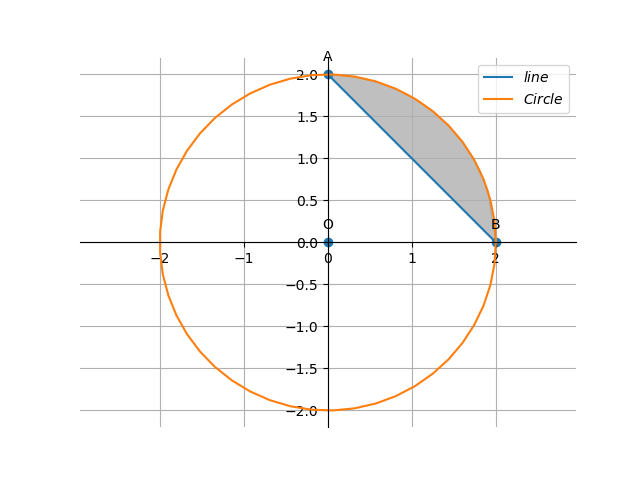
\includegraphics[width=1\columnwidth]{./figs/conic.png}
\caption{Smaller region between Circle and Line}
\label{fig:conic}
\end{figure}

\raggedright \textbf{Given}: \\
Equation of circle is  
\begin{equation} x^2 + y^2 = 4
\end{equation}
Equation of line is 
\begin{equation}
x+y=2
\end{equation}
\textbf{To Find:} \\
To find the intersection points and area of shaded region shown in figure\
\section{Construction}

\begin{table}[h!]
\begin{center}
\setlength{\arrayrulewidth}{0.5mm}
\renewcommand{\arraystretch}{1.5}
    \begin{tabular}{|l|c|}
    \hline 
    \textbf{Points} & \textbf{coordinates} \\ \hline
   $\vec{A}$ & $\myvec{
   0\\
   2
   } $ \\\hline
   $\vec{B}$ & $\myvec{
   2\\
   0
   } $ \\\hline
      \end{tabular}
  \end{center}
\end{table}
\newpage
\section{solution}
The given circle can be expressed as conics with parameters,
\begin{equation}
\vec{V}=\myvec{
4 & 0\\
0 & 4
}
\end{equation}
\begin{equation}
\vec{u}=0 
\end{equation}
\begin{equation}
f=-16
\end{equation}

The given line equation can be written as\\ 
\begin{align} 
	\vec{x}=\begin{pmatrix}2 \\ 0 \\ \end{pmatrix}+k\begin{pmatrix}\frac{1}{2} \\ -\frac{1}{2} \\ \end{pmatrix}
\end{align}
The points of intersection of the line, \\ 
\begin{equation}
L: \quad \vec{x} = \vec{q} + \kappa \vec{m} \quad \kappa \in \mathbb{R}
\end{equation}

with the conic section, \\ 
\begin{align}
	\vec{x}^{\top}\vec{V}\vec{x} + 2\vec{u}^{\top} \vec{x} + f = 0
\end{align}
are given by \\
\begin{align}
\vec{x}_i = \vec{q} + \kappa_i \vec{m}
\end{align}
where, \\

\begin{equation*}
\kappa_i = \frac{1}
{
\vec{m}^T\vec{V}\vec{m}
}
\lbrak{-\vec{m}^T\brak{\vec{V}\vec{q}+\vec{u}}}
\pm
\end{equation*}
\begin{equation}
\rbrak{\sqrt{
\sbrak{
\vec{m}^T\brak{\vec{V}\vec{q}+\vec{u}}
}^2
-
\brak
{
\vec{q}^T\vec{V}\vec{q} + 2\vec{u}^T\vec{q} +f
}
\brak{\vec{m}^T\vec{V}\vec{m}}
}
}
\end{equation}
On substituting\\
\begin{align}
\vec{q} &= \myvec{
2\\
0
} 
\end{align}
\begin{align}
\vec{m} = \myvec{\frac{1}{2} \\ -\frac{1}{2}}
\end{align}
With the given as in eq(3),(4),(5),\\ 

The value of $\kappa$ ,\\
\begin{equation}
\kappa =0,-4
\end{equation}
    
by substituting eq(13) in eq(6) we get the
points of intersection of line with ellipse \\
\begin{align}
    \vec{A}=\myvec{
0\\
2
    }
\end{align}
\begin{align}
    \vec{B}=\myvec{
2\\
0
    }
\end{align}
From the figure \\
Total area of portion is given by,\\ 
Total Area=(area of circle in first quadrant)-(area of a triangle \textbf{AOB})

\subsection*{Area of triangle}

\begin{align}
\implies A_1=\int_{0}^{2} (2-x) \,dx
\end{align}
by solving the above equation we get area of triangle as 2 units
\subsection*{Area of circle}

\begin{align} 
\implies A_2=\int_{0}^{2}\sqrt{4-x^2} \,dx 
\end{align}
by solving the above equation we get area of circle $\pi$

the total area is
$\implies \vec{A}=\pi - 2$


\begin{table}[h]
\large
\begin{tabular}{lll}
\multicolumn{3}{l}{Get Python Code for image from}                                                 \\ \hline
\multicolumn{3}{|l|}{\url{https://github.com/ManojChavva/FWC/blob/main/Matrix/conics/code/conic.py}} \\ 
 \hline
\multicolumn{3}{l}{Get LaTex code from}                                                            \\ \hline
\multicolumn{3}{|l|}{\url{https://github.com/ManojChavva/FWC/blob/main/Matrix/conics/conic.tex}}            \\ \hline
\end{tabular}
\end{table}



\end{document}




